\documentclass[12pt,a4paper]{article}
\usepackage[]{listings}
%packages used
\usepackage[english]{babel}
\usepackage[margin=1in,  left=1.25in]{geometry} %margins
\usepackage{pslatex}%Times new roman font
\usepackage{graphicx}%for images
\usepackage{float}
%\usepackage{fancyhdr}
%\pagestyle{fancy}
%\fancyfoot{}

%beginning of document
\begin{document}
%declaration page
%\thispagestyle{empty}
\pagenumbering{roman} 
\begin{titlepage}
  \begin{center}
    \vspace*{1cm}

    \textbf{\Huge Cache report}

    \vspace{0.5cm}

         
    \vspace{1.5cm}

    \textbf{\large Chang Zihao \\20206018\\\large Cui Yuxuan\\20206019}

    \vfill
         

         
    \vspace{0.8cm}
  


         
\end{center}
\end{titlepage}


\newpage
%table of contents
\tableofcontents
\thispagestyle{empty}

\newpage
\pagenumbering{arabic}
\setcounter{page}{1}

\section{Introduction}

Lab5 is required to design a Cache.
A cache processes three state--read and hit, read but miss, and write.
And use cache to save data that use much to save time.
We use multi cycle CPU link the cache.

\subsection{Read Data}

\begin{enumerate}
\item Processor send the address to the cache
\item Then use the valid digit and sign digit to find the data.
\item If the data exist then hit, and send the data to the processor.
\item If the data does not exist then send miss to the memory, the memory will send the data that according to the requirement to the specific position.

\end{enumerate}

\subsection{Write data}

\begin{enumerate}
\item Memory send the address and the data to the cache
\item Then compare the valid digit and sign digit to find the specific position in the cache.
\item Write in the data.

\end{enumerate}

\newpage

\section{Design}

As the Description of TB file mentioned, We do not need to implement memory and register ourselves.
So we design the path to connect them together.

\subsection{Module design}
\begin{enumerate}
\item Write-through
\item Write-allocate
\item Blocking cache
\end{enumerate}
\newpage

\section{Implementation}

%The whole circuit was shown below.

%\begin{figure}[H]
 % \centering
 % \includegraphics[height=5in, angle=90]{datapath.JPG}
 % \end{figure}
%There might be something different with the circuit.
%  \begin{figure}[H]
%    \centering
%    \includegraphics[height=3.5in]{cont.jpg}
%    \end{figure}
\newpage

\section{Evaluation}

I pass all the test in the testbench folder.

\begin{figure}[H]
  \centering
  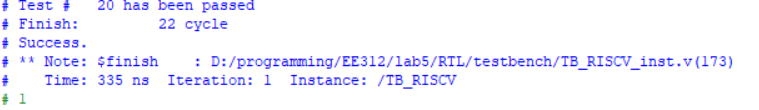
\includegraphics[height=3in]{inst.png}
  \end{figure}

\begin{figure}[H]
  \centering
  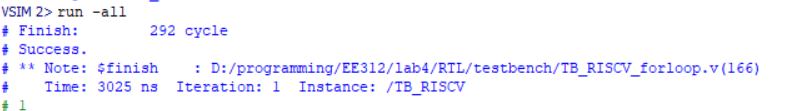
\includegraphics[height=3in]{forloop.png}
  \end{figure}

  \begin{figure}[H]
    \centering
    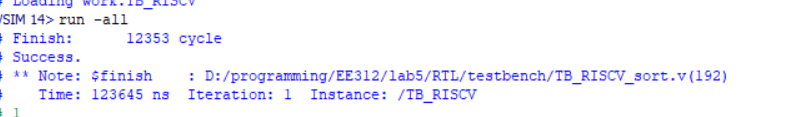
\includegraphics[height=3in]{sort.png}
    \end{figure}

% We first encountered some problems in understanding the meaning of the question, 
% but in the end by looking at the test code, 
% we thoroughly understood the meaning of the question.
% And at last, we pass all the test and finished the whole project.
% I hope that future projects will give enough time to think and complete the code.

\section{Conclusion}

The cache is very useful in the CPU nowadays,it make the CPU quicker than the CPU last few years.
\end{document}
